\chapter{Proximity Computations on Streaming Noisy Sensor Data}
\label{chp:PCollide2}


\section{Introduction}

In this chapter, we continue addressing
the issue of collision detection and distance computation on point cloud data generated from robot sensors. However, unlike Chapter~\ref{chp:PCollide}, we focus more on the sensor data streams.
This includes data streams provided by visual sensors that can compute depth information in the form of a point cloud (e.g., laser sensors, stereo
cameras, time-of-flight cameras). We assume these
sensors periodically generate point cloud data corresponding to their
field of view. We call each view of the environment a ``frame'' of the stream.

The generated point clouds correspond to samples on the visible parts
of the various objects in the environment. Dealing with these samples
of the environment introduces many challenges: 1) it can be expensive
to extract objects from the sensor data because such operations involve
complex steps such as segmentation~\cite{Rusu:2009:IROS} or object
recognition~\cite{Muja:2011:ICRA}, among others; 2) tracking objects
among different frames of sensor data is challenging due to noise and
amount of sensor data; 3) amount of sensor data is large and is typically
received at high frame rates; for example, typical RGB-D sensors like
the Microsoft Kinect\texttrademark{}  sensor can generate a detailed point
cloud with around 300,000 points at 30 Hz; and 4) sensor data usually
contains some level of noise and uncertainty and may not represent
the environment fully (some parts are occluded). However, most
collision and distance computation algorithms assume that a geometric
model for each object in the environment is available. Furthermore,
there are two additional issues in terms of applying existing
algorithms to dynamically generated sensor data. First, most proximity
algorithms tend to compute complex acceleration data structures before
performing actual queries. The computational overhead of such data structures can be high for large sensor data. Second, parts of the environment are not well captured by the sensor data. In
traditional approaches such regions are considered either as
free space (optimistic, but unsafe) or as occupied (safe, but perhaps
too conservative). Instead, we need techniques that model the uncertainty in the captured point-cloud data.

In this chapter, we present real-time collision detection and distance
computation algorithms for point cloud sensor data stream.  Our approach is
general and is applicable to all sensors that can generate point clouds.
Given one point cloud frame, we first convert it into an octree, a
compact data structure for modeling arbitrary environments, which can encode
the uncertainty in the sensor data and in the occluded
space~\cite{octomap}. Based on the octree representation, we present
two techniques to perform efficient collision and distance queries on
the sensor data:
\begin{itemize}
\item We amortize the cost of initialization over multiple or all
  proximity queries. That is, we initialize the acceleration data structure (a dynamic AABB tree) for
  collision or distance queries using a simple technique
  that is not optimal but fast, and then we incrementally improve the tree's quality as more proximity queries are performed.
\item In the second strategy, we completely avoid the initialization
  overhead by performing collision and distance queries directly with
  the octree representing the sensor. In this case, each query
  may be slightly more expensive than using traditional methods. However, we save the overhead of computing a spatial data structure that is used to accelerate the queries.
\end{itemize}

These two strategies are complementary and used in different settings. Each of them can provide up to an order of magnitude improvement over prior methods for proximity computations over sensor data. In order to handle occlusions and uncertainty in sensor data, our new algorithms assume that each leaf
node in the octree specifies a probability of
occupancy~\cite{octomap}. As sensor data is received, the probability of
occupancy is maintained to be an average of occupancy over a number of
previously observed frames. Our
approach uses the probability of occupancy specified in the octree and
can report a set of axis-aligned bounding boxes, that
correspond to intersections of robot links and octree nodes. These
bounding boxes also specify the probability of occupancy carried over
from the octree node. Using this set of bounding boxes, a notion of
cost can be defined for collision detection. A simple example of cost is the
weighted sum of the box volumes using the probabilities of occupancy
as weights.

We validate the performance of our new algorithms on both synthetic
sensor data and real sensor data generated with a RGB-D sensor.
The algorithms are implemented in the open source library
FCL~\cite{Pan:ICRA:2012}.

The rest of this chapter is organized as follows. We survey related work
on collision checking and distance computation on sensor data in
Section~\ref{sec:8:related}. Section~\ref{sec:8:overview} explains why
previous methods are not efficient for sensor data streams and gives an
overview of our new methods. Section~\ref{sec:8:algorithm} discusses the
details of our new approaches. We present the results in
Section~\ref{sec:8:result}.


\section{Problem Definition and Related Work}
\label{sec:8:related}

The general collision query is defined as follows:

\emph{Given two sets of objects $\{A_i\}_{i=1}^n$ and
  $\{B_i\}_{i=1}^m$ with $n$ and $m$ objects, respectively, as well as
  their configurations, the collision detection query returns a yes/no
  answer about whether any pairs of objects, one from each set, are in
  collision with each other. Optionally, it also returns all pairs
  of colliding objects.}

A special case of the collision query is when the two sets of objects
are the same, which is called the self-collision query. As an example,
a self collision check is useful to test whether a configuration of an
articulated model is valid.

The general distance query is defined as follows:

\emph{Given two sets of objects $\{A_i\}_{i=1}^n$ and
  $\{B_i\}_{i=1}^m$ with $n$ and $m$ objects, respectively, as well as
  their configurations, the distance query returns the minimum separation distance
  between the two sets. Optionally, it also returns the pair of
  objects that are closest to each other.}

In order to avoid the quadratic worst-case complexity of collision checking or distance computation between two sets of objects, prior
techniques use a two-phased approach: a broad phase and a narrow
phase. Intuitively, broad-phase computation excludes object pairs
that definitely are not colliding or are far away, and identifies
the pairs of objects that may be colliding or may contribute to the
minimum distance between the two
sets~\cite{Eric2004book,Pan:ICRA:2012}. The narrow-phase computation
corresponds to exact, pairwise collision or distance tests between the identified pairs.

To efficiently cull out object pairs that are definitely not colliding
or are far away, special data structures are used to manage all
the objects in the given set. For example, interval
trees~\cite{Tracy:2009:ELS} are used in sweep-and-prune (SaP) based broad-phase algorithms; spatial partitioning trees such as octrees and $k$-d
trees can also be used~\cite{Bandi:1995}; hash tables are used in
spatial-hashing based approaches~\cite{Eric2004book}.  SaP is essentially a dimension reduction
approach in which objects are projected into a lower dimension
and then overlap tests are performed by sweeping a hyperplane along the dimensional axis.
In spatial-hashing, objects are registered into some form of grid, and collision tests are performed
locally inside the grid cells. SaP is effective when moving objects have
a high spatial coherence while spatial-hashing is effective for objects of similar size.
These broad-phase data structures are designed so they can be updated efficiently when the
underlying objects change their positions or when objects are added
into or removed from the environment. In traditional broad-phase
approaches, the overhead to initialize the broad-phase data structure
is usually ignored, because the broad-phase data structure is
typically used for a long time over many queries. As a result, the
initialization overhead is negligible when compared to the total time
of a large number of collision or distance queries performed by the
underlying application.

Previous work on proximity queries on sensor data tends to ignore the
fact that the underlying data can be updated quickly when a new frame
is received from the sensor. For example, the
sensor data is first converted into a set of boxes~\cite{Rusu:RPG:2009}, and then ODE~\cite{ODE} is used to check for collisions between these
boxes and the robot. Passing the sensor data to the collision checker
in this manner is relatively slow when the frame rate of the sensor is
high.

Some recent work attempts to handle collision checking with sensor
data in a more sophisticated manner. For real-time haptics rendering,
Leeper et al.~\cite{Leeper:ICRA:2012} represent the point cloud using
an implicit surface and use that implicit surface for collision
checking. The accuracy of this method depends on the parameters used for
the implicit surface fitting.


\section{Overview}
\label{sec:8:overview}

Current collision detection algorithms make assumptions that may no
longer hold when dealing with data from real sensors.
All existing methods require their inputs in terms of a set of \emph{objects}.
An object is defined as a collection of geometric elements (points, triangles,
etc) that have a well-defined boundary~\cite{Alexe:2010:CVPR} -- for
example, a desk, a cup on the desk, etc.  In synthetic environments,
the objects are provided by default, in the form of meshes or
geometric primitives. However, for sensor data, the entire environment
is in the form of a single point cloud, and different objects
contained in the environment are not easily separable in the point
cloud. To extract objects from the point cloud, expensive object
recognition and reconstruction algorithms, such
as~\cite{Muja:2011:ICRA}, are necessary. To bypass such difficulties,
one widely used solution is to discretize the space that contains the points into small axis-aligned cubes and model the sensor data as a collection of boxes with localized points. This representation is referred to as
a \emph{collision map} in~\cite{Rusu:RPG:2009,Ioan:2010}. After
converting the sensor data to a set of boxes, the collision or
distance query between the robot and the environment becomes a query
between the robot and the set of boxes. Broad-phase structures for
both the robot and for the boxes can be constructed before performing
actual queries.  A diagram of this pipeline (used in~\cite{Rusu:RPG:2009,Ioan:2010}) is shown in
Figure~\ref{fig:8:pipelines}(a).

In pipelines such as ones presented in~\cite{Rusu:RPG:2009}
and~\cite{Ioan:2010}, the raw sensor data in the form of point
clouds is first converted into a collision map structure.
We denote the time required to construct the collision map as $T_0$,
which is small compared to the timing cost of other components in the
pipeline. It takes time $T_1$ to convert the collision map into a data
structure suitable for broad-phase approaches, which includes two
parts: 1) $T_{1,1}$: the time cost from collision map to boxes; 2)
$T_{1,2}$: the time cost from boxes to broad-phase
structures. $T_{1,2}$ can be expensive if the sensor data is large and
there are many boxes. For example, the PR2 stereo sensor data usually
contains tens of thousands of points and is converted to thousands of
boxes. An additional challenge is that these generated data structures
cannot be easily reused when new sensor data comes in, as is
assumed by traditional approaches.
This is because the boxes
managed by the structure are not trackable objects: they are just
spatial cells that contain several points belonging to one frame of
the sensor data. Given a new frame of sensor data, it is difficult to
identify each box's correspondence in the prior frames; traditional approaches depend on the easily-identified correspondence to prior frames in order to compute the objects' movements and update the broad-phase structure accordingly. Therefore, once a
new frame of sensor data is received, we need to discard the old broad-phase structure and reconstruct a new one from scratch. Moreover, as
the sensor data is received at high frame rates (e.g., Kinect\texttrademark{} frame
rates can be 30 Hz and the stereo sensors on PR2 generates data at 20
Hz), we can only perform a few
(e.g., $N < 1,000$) queries during the lifetime of a broad-phase
structure. As a result, for sensor data it is possible that:
\begin{equation}
T_1 = T_{1,1} + T_{1,2} \ \ \sim \ \ T_2 = N \cdot T_q,
\end{equation}
where $T_q$ is the time cost for a single query. In other words, the overhead to process the sensor data for queries can be comparable to the total time spent on the actual queries and is in fact not negligible.

According to the analysis above, the overall time to handle one
frame of sensor data is:
\begin{equation}
\label{eq:8:overalltime}
T = T_0 + T_1 + T_2 = T_0 + T_{1,1} + T_{1,2} + N \cdot T_q.
\end{equation}
To improve performance for large point cloud datasets, we provide two strategies. The first
strategy reduces the broad-phase structure construction time
$T_{1,2}$ by amortizing the cost over all the $N$ queries. We first
construct a low-quality broad-phase structure, which is less effective
in culling but is much faster than the near-optimal broad-phase
structure used before, i.e., the new construction time is
$\widetilde{T}_{1,2} \ll T_{1,2}$. When performing the actual queries,
we can improve the broad-phase structure gradually with each
query. The new broad-phase structure can slow down the actual queries
because we may perform more narrow-phase computations, i.e.,
$\widetilde{T}_q > T_q$. However, the incremental refinement of the broad-phase structure guarantees that over the long term with many queries, there may be no overall decrease in performance. As long as $T_{1,2} + N \cdot T_q > \widetilde{T}_{1,2} + N
\cdot \widetilde{T}_q$, i.e.,
\begin{equation}
\label{eq:8:Nstrategy1}
N \leq \frac{T_{1,2} - \widetilde{T}_{1,2}}{\widetilde{T}_q - T_q},
\end{equation}
the amortized method will be faster than the original method.

The second strategy is to support collision or distance queries
directly, using the octree directly provided by the sensor data. This means that we no longer need a broad-phase structure to manage the sensor data. As shown in Figure~\ref{fig:8:pipelines}(b), this approach does not compute any data structures and overcomes the overhead $T_1$. However, because this approach uses the octree as a low-quality
broad-phase structure, the performance of actual collision/distance queries may slow somewhat. Suppose the time for actual query in this case
is $\widetilde{T}_q^\prime$, then the second strategy is better than
previous methods if $N \leq \frac{T_{1,2}}{\widetilde{T}_q^\prime - T_q}$.

Both these strategies can be extended to handle sensor data with
uncertain or unknown regions. The octree represents an uncertain or
unknown region as a octree leaf node with an occupancy probability
smaller than $1$~\cite{octomap}. When using the first strategy, the
boxes generated can store an occupancy probability with them, which
will be considered in the narrow-phase algorithms. If the second
strategy is used, the octree's occupancy probability will directly be
involved when performing collision or distance queries with the
octree structure.


\begin{figure*}[htbp]
\centering
\subfloat[Pipeline for collision or distance
  computation: The sensor data is first represented as a collision
  map constructed in $T_0$ time. Next, the
  collision map is first converted into a set of boxes in $T_{1,1}$
  time. Finally, a broad-phase data structure is constructed in
  $T_{1,2}$ time in order to manage these boxes. The overhead to
  prepare the sensor data is $T_1 = T_{1,1} + T_{1,2}$. Once the data
  is prepared, the actual time to perform $N$ collision or distance
  queries is $T_2 = N \cdot T_q$, where $T_q$ is the time cost for a
  single query. In traditional approaches, $N$ is assumed to be
  infinite, while for sensor data, $N$ is usually small ($<$ 1,000).]
          { 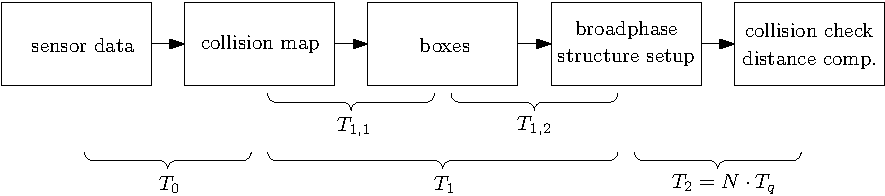
\includegraphics[width=0.8\linewidth]{figs/8/pipeline.pdf}
  \label{fig:8:pipeline}
}

\subfloat[By supporting the collision or distance
  query directly with the sensor data represented as an octree, we no
  longer need the long conversion pipeline from octree to broad-phase
  structures and thus can completely avoid the main overhead $T_1$.] {
  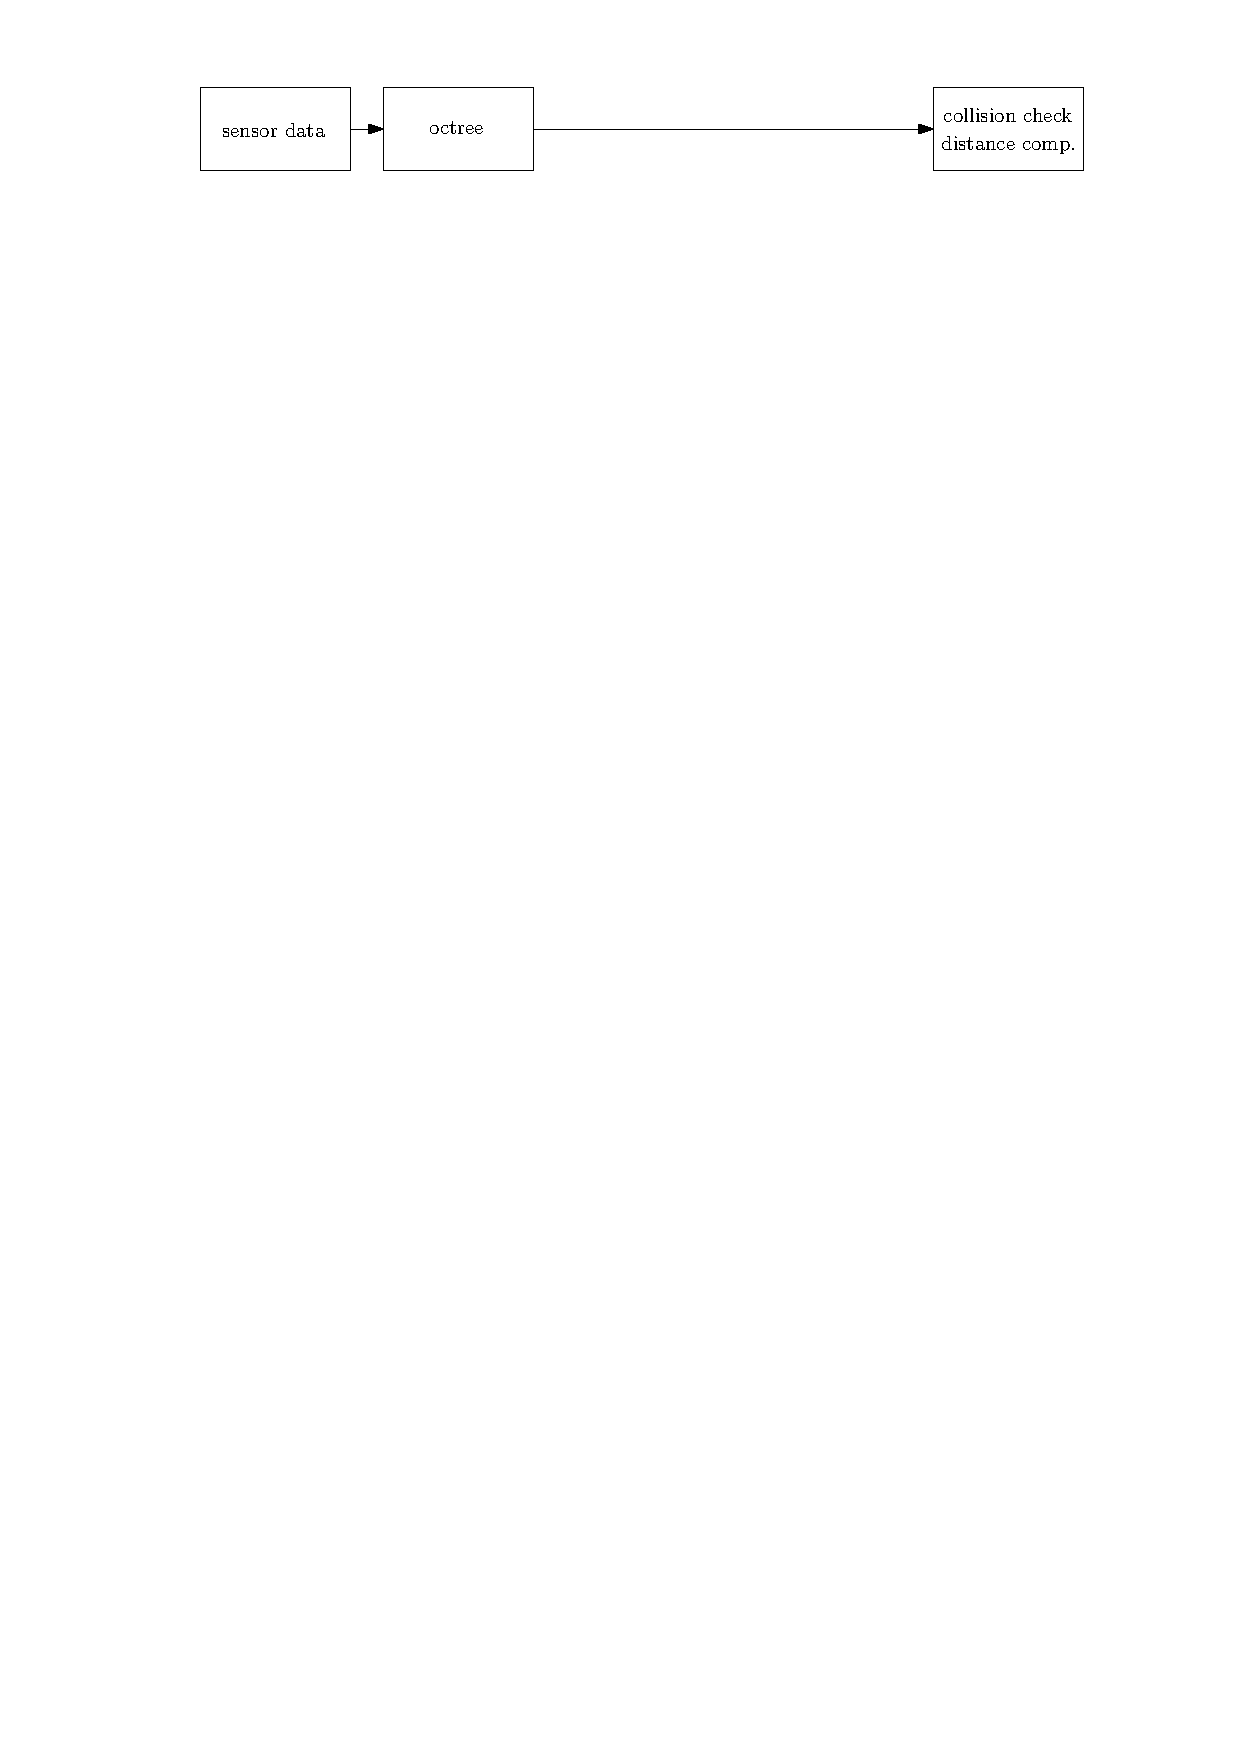
\includegraphics[width=0.8\linewidth]{figs/8/newpipeline.pdf}
  \label{fig:8:newpipeline}
}
\caption[Comparison between possible pipelines for environment representation and collision detection]{\label{fig:8:pipelines} Comparison between possible pipelines for environment representation and collision detection.}
\end{figure*}


\section{Efficient Collision and Distance Queries on Sensor Data}
\label{sec:8:algorithm}

In this section, we discuss the details of our new algorithms,
which are optimized to handle sensor data. In all the descriptions that follow,
we use the \emph{dynamic AABB (Axis Aligned Bounding Box) tree} as the default broad-phase data structure to manage all the boxes converted from sensor data in the form of an octree or collision map. We remind the readers that a dynamic AABB tree is a binary tree
structure used to organize objects in a hierarchical manner. The dynamic AABB tree recursively splits a set of objects into two subsets; this process continues until the set contains only one object and is used as a leaf node. Previous methods try to construct a high-quality AABB tree in order to perform broad-phase culling effectively, e.g., the split axis is selected to minimize the
bounding boxes of the children nodes. When new objects
are added to or old objects are removed from the tree, the dynamic AABB tree must be
re-balanced and the tree structure must be adjusted to minimize the bounding volume of
each tree node. Such re-balancing operations are also necessary when
objects have moved. The time complexity to construct a balanced dynamic AABB tree is $\mathcal
O(n \log n)$ where $n$ is the number of objects managed by the
tree. This is because the tree has $\log n$ levels and each level
needs $\mathcal O(n)$ time to rearrange the objects. If $n$ is large,
this construction step can be expensive. For sensor data, $n$ is the number of boxes computed from sensor data and can be as high as 10,000.

\subsection{Amortized broad-phase Algorithm}
Our first method attempts to reduce the construction time of a dynamic
AABB tree, i.e., $T_{1,2}$ in Equation~\ref{eq:8:overalltime}. Instead
of constructing a high-quality dynamic AABB tree, we start with a low-quality binary tree and then gradually improve it during the following
actual queries. The initial binary tree is constructed by using the
well known space-filling Morton curve~\cite{Morton:1966} -- also known as the Lebesgue
and z-order curve -- to order all the boxes converted from the sensor data. We assume that the
enclosing AABB of the entire environment is known. We take the
barycenter of each of the $n$ boxes as its representative point. By
constructing a $2^k \cdot 2^k \cdot 2^k$ lattice within the enclosing
AABB, we can quantize each of the three coordinates of the
representative points into $k$-bit integers. The $3k$-bit Morton code
for a point is computed by interleaving the successive bits of its
quantized coordinates. Figure~\ref{fig:8:morton} shows a 2D-example of
this construction. Sorting the representative points in increasing
order of their Morton codes will lay them out in order along the
Morton curve. Therefore, it will also order the corresponding boxes
in a spatially coherent way, which directly determines a binary tree
structure for the set of boxes. The time cost of this new tree
construction method is dominated by the time to sort $n$ $3k$-bit
integers, which is of time complexity $\mathcal O(3k \cdot n)$ if we
use radix sorting. If $k$ is smaller than $\log n$, the Morton curve
based construction method is cheaper than the traditional AABB tree
construction method. Moreover, $k$ also enables us to control the
quality of the resulting initial tree: we can obtain broad-phase
structure with better culling efficiency by using larger $k$.

The AABB tree constructed as above may not be as effective at culling
as the high-quality AABB tree constructed with traditional approaches and therefore the timing cost of each actual query can increase, i.e., $T_q$ item in Equation~\ref{eq:8:overalltime}
can be larger. To overcome this problem, our solution is to
incrementally refine the initial binary tree while performing each
query. First, we encode each traversing path
connecting the tree root node to one of the leave nodes as an $\mathcal
O(\log n)$-bit integer, according to whether the left or right child
is selected during the traverse. Next, while performing the actual query, we
periodically select one of the traversing paths and re-compute the
bounding boxes for all the nodes on the path. We begin from the leaf
node, which has time complexity $\mathcal O(\log n)$. Then after (at most) $n$ iterations, the binary tree will become an AABB tree that is able to cull effectively. In practice, we have observed that the dynamic
tree's culling efficiency can be almost as good as the near-optimal
binary tree in only a few iterations. As a result, we can assume that the
actual query cost when using the amortized method is $\widetilde{T}_q
= T_q + \mathcal O(\log n)$.

Suppose $N$ queries are performed during the lifetime of the dynamic
AABB tree. Then, according to Equation~\ref{eq:8:overalltime},
if $N < \frac{c_1 \cdot n \log n - c_2 \cdot 3 k \cdot n}{c_3 \cdot \log n}$, the amortized method will have better
performance than the traditional methods. Here $c_1$, $c_2$ and $c_3$ are constant coefficients for $\mathcal O(n\log n)$, $\mathcal O(3k \cdot n)$ and $\mathcal O(\log n)$: $c_1$ is the cost to place a given AABB on one side of an axis-aligned plane according to its center coordinates; $c_2$ is cost to decide whether to exchange the position of two $3k$-bit integers by comparing one of the $3k$ bits; $c_3$ is the cost to test whether a given AABB is completely within another AABB and if not, enlarge the second AABB. For $c_3 > c_1 > c_2$, we have that the above upper bound for $N$ can be approximated by $N < \frac{c_1}{c_3} n$.

\begin{figure}[htbp]
\centering
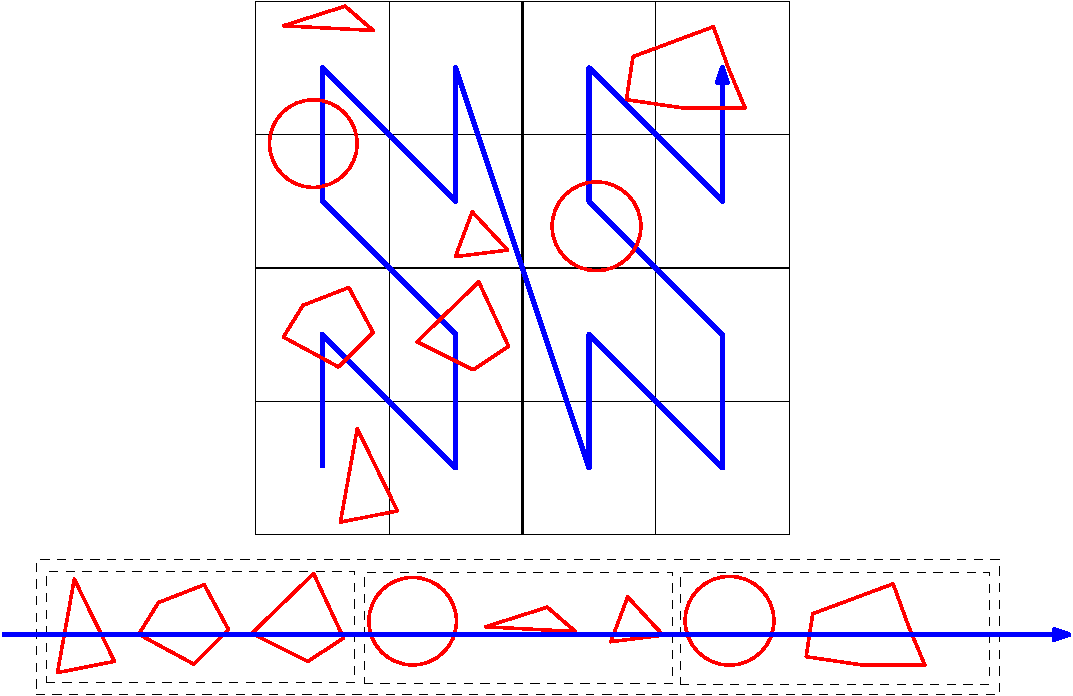
\includegraphics[width=0.8\linewidth]{figs/8/morton.pdf}
\caption[Illustration of 2-D Morton curve]{\label{fig:8:morton} Example of 2-D Morton curve. According to the first two
bits of the Morton code, we can order the objects in a hierarchical manner.}
\end{figure}


\subsection{Proximity Computation using Octrees}
The amortized method cannot avoid the overhead of $T_{1,1}$ in Equation~\ref{eq:8:overalltime}, which can still be expensive for large sensor data.
To avoid such overhead, our second method
performs proximity queries directly on the sensor data in
the form of an octree (as shown in Figure~\ref{fig:8:pipelines}(b)); this completely avoids the long pipeline shown in (Figure~\ref{fig:8:pipelines}(a)) required to prepare sensor
data. In other words, we use the octree as a low-quality broad-phase
structure for the sensor data. Octrees may not be as efficient at
culling as a dynamic AABB tree, so the cost for a single collision or
query cost can be larger than using the traditional pipeline, i.e.,
$\widetilde{T}_q^\prime > \widetilde{T}_q > T_q$. However, as
only a small number of queries are performed for one frame of sensor
data, the saving on sensor data preparation time may make this
strategy more efficient than the amortized strategy.




\begin{algorithm}[htb]
	\caption{\texttt{collisionRecurse}$(\texttt{node}_1, \texttt{node}_2)$}
	\label{algo:collision_recurse}
	\begin{algorithmic}[1]
      \IF{$\texttt{node}_1.\texttt{isLeaf()}$ $\texttt{and}$ $\texttt{node}_2.\texttt{isLeaf()}$}
           \IF{\texttt{overlap}$\texttt{(node}_1.\texttt{bv}, \texttt{node}_2.\texttt{bv)}$}
                \STATE narrow-phase collision between the octree box in \texttt{node}$_1$ and the object in \texttt{node}$_2$
           \ENDIF

           \RETURN collision status
      \ENDIF

         \IF{$\texttt{node}_2.\texttt{isLeaf()}$ $\texttt{or}$ $(\texttt{node}_1.\texttt{hasChildren()}$ $\texttt{and}$ $\texttt{node}_1.\texttt{bv} > \texttt{node}_2.\texttt{bv})$}
              \FOR{$i = 1$ \TO $8$}
                \IF{$\texttt{node}_1.\texttt{child(i).occupancy\_prob()}$ $>$ $\texttt{threshold}$}
                   \STATE  \texttt{collisionRecurse}$\texttt{(node}_1.\texttt{child(i)}$, $\texttt{node}_2\texttt{)}$
                \ENDIF
              \ENDFOR
            \ELSE
              \STATE \texttt{collisionRecurse}$\texttt{(node}_1$, $\texttt{node}_2.\texttt{leftChild())}$
              \STATE \texttt{collisionRecurse}$\texttt{(node}_1$, $\texttt{node}_2.\texttt{rightChild())}$

            \ENDIF
\end{algorithmic}
\end{algorithm}



\begin{algorithm}[htb]
	\caption{\texttt{distanceRecurse}$(\texttt{node}_1, \texttt{node}_2, d_{\text{min}})$, $\texttt{node}_1$ is one node of the octree structure, and $\texttt{node}_2$ is one node from the other binary tree structure that is used to perform distance computation with the octree. $d_{\text{min}}$ keeps the minimum distance computed till now and is initialized to be $\infty$. The second tree structure can represent a dynamic AABB tree working as the broad-phase structure for all the links of an robot, or an OBB tree for one mesh, or even a single geometric shape (i.e., a tree with only one node). }
	\label{algo:distance_recurse}
    \begin{algorithmic}[1]
      \IF{$\texttt{node}_1.\texttt{isLeaf()}$ $\texttt{and}$ $\texttt{node}_2.\texttt{isLeaf()}$}
           \STATE $d \leftarrow$ narrow-phase distance between the octree box in \texttt{node}$_1$ and the object in \texttt{node}$_2$
           \STATE $d_{\text{min}} \leftarrow \min(d, d_{\text{min}})$
           \RETURN
      \ENDIF

         \IF{$\texttt{node}_2.\texttt{isLeaf()}$ $\texttt{or}$ $(\texttt{node}_1.\texttt{hasChildren()}$ $\texttt{and}$ $\texttt{node}_1.\texttt{bv} > \texttt{node}_2.\texttt{bv})$}
              \FOR{$i = 1$ \TO $8$}
                \IF{$\texttt{node}_1.\texttt{child(i).occupancy\_prob()}$ $>$ $\texttt{threshold}$}
                     \IF{\texttt{distance}$\texttt{(node}_1.\texttt{bv}, \texttt{node}_2.\texttt{bv)} < d_{\text{min}}$}
                       \STATE \texttt{distanceRecurse}$\texttt{(node}_1.\texttt{child(i)}$, $\texttt{node}_2$, $d_{\text{min}})$
                     \ENDIF
                \ENDIF
              \ENDFOR
            \ELSE
              \STATE \texttt{distanceRecurse}$\texttt{(node}_1$, $\texttt{node}_2.\texttt{leftChild()}$, $d_{\text{min}})$
              \STATE \texttt{distanceRecurse}$\texttt{(node}_1$, $\texttt{node}_2.\texttt{rightChild()}$, $d_{\text{min}})$
            \ENDIF
\end{algorithmic}
\end{algorithm}


We will now illustrate the use of this algorithm to perform collision
checking between an articulated
robot and the sensor data. The desired query can be implemented as a collision
query between trees: the sensor data is represented as an octree and
the robot is represented as a binary dynamic AABB tree. The algorithm
is shown in Algorithm~\ref{algo:collision_recurse}, which is a
recursive method. We start with two root nodes of the two trees. If
both of them are leave nodes, we perform the narrow-phase collision
between the object corresponding to the given dynamic AABB tree node
and one cubic cell in the octree. Otherwise, we need to check for
collisions between the subtrees rooted at the corresponding two nodes. If the
given octree node is not a leaf node, we recursively perform collision queries
between the given dynamic AABB
node and each of its eight children nodes. Otherwise, we recursively perform collision queries between the given
octree node and the two children of the given dynamic AABB node. The
recursion continues until the collision is detected. One major issue is mentioned in Algorithm~\ref{algo:collision_recurse} at line $8$: we only perform
collision queries for octree cells with occupancy probabilities larger than a
given threshold. This is because the octree representation of the sensor data can encode uncertain or
unknown regions in the environment, and we want the result computed by
the new method to be consistent with the result provided by the simpler
pipeline in Figure~\ref{fig:8:pipelines}(a), where octree cells are
converted into boxes only if their occupancy probability is larger
than a given threshold.

Similar recursive traversal can be used to handle the distance
query between the robot and sensor data. Moreover, a binary tree
can also be used to represent other types of data; e.g., a mesh can be
represented as a binary AABB or OBB tree~\cite{Pan:ICRA:2012} and a
geometric primitive (e.g., a sphere) can be represented as a binary
tree with only the root node. As a result, the same recursive formulation can be used to handle the proximity query between the sensor data and
either a mesh or a geometric primitive.


\subsection{Collision Checking with Uncertain/Unknown Regions}
The data gathered by various sensors tend to have error and noise.
Many sensors only have limited precision, which results in sampling
error in the sensor data. Often, part of the environment may not be
observed by the sensor, because sensors only have limited field of
view and may have a large blind spot. Moreover, the camera or laser
may not be perfectly calibrated; thus the generated point clouds
may have systematic bias. It is important to handle the uncertain or
unknown part of the sensor data so that robots can work robustly in
real world scenarios.

The unknown or uncertain regions are usually assumed to be
collision-free, e.g., such an optimistic assumption is made
in~\cite{Rusu:RPG:2009}. This assumption can cause serious problems in some
cases. In the example shown in Figure~\ref{fig:8:unknowncollision}(a), the sensor
mounted on the robot's head cannot cover the region near the robot's
left arm. Therefore, given a path for the left arm moving
through the unknown region, the collision checking routine will always
assume it to be collision-free, even if obstacles exist in that
region. Our solution here is to compute a set of
boxes representing different regions in the unknown space that
intersect with the swept volume of the robot's path. Only boxes
with the largest occupancy probability are returned, because they are
the most important regions to check when determining whether the given path is
collision free. Given these boxes as shown in Figure~\ref{fig:8:unknowncollision}(b), users can implement different
strategies according to different applications. For example, the robot
can try to avoid the unknown regions completely, minimize its motion
through the unknown regions or actively sense the unknown regions to
gain more information about them.

The intersection between the unknown space and the swept volume of the
robot's path can be performed by checking the collisions between
the octree and a series of samples on the path. Each collision
query can be performed based on a recursive method similar to Algorithm~\ref{algo:collision_recurse}. %However, in this approach, we won't include the occupancy check shown in line $8$, because we need to consider the unknown and uncertain octree cells besides the cells that are definitely occupied.

\begin{figure}[htbp]
\mbox{
\subfloat[Collision checking only performed between the planned trajectory and the regions that are known to be occupied (the blue part) in the sensor data.]
{
  \centering
  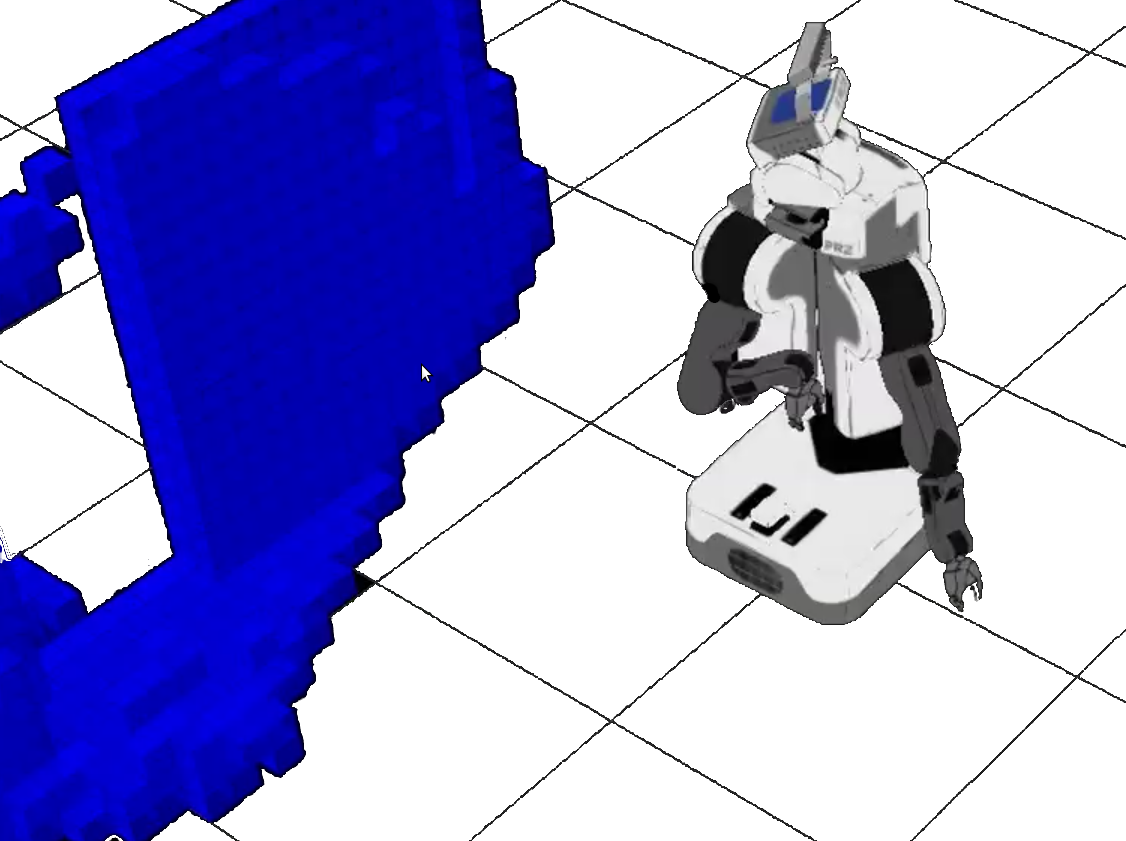
\includegraphics[height=2.1in]{figs/8/unknown.png}
  \label{fig:8:unknown}
}
\quad
\subfloat[Collision checking is performed between the planned trajectory and both
the regions that are known to be occupied (the blue part) and the unknown regions in the sensor data.]
{
  \centering
  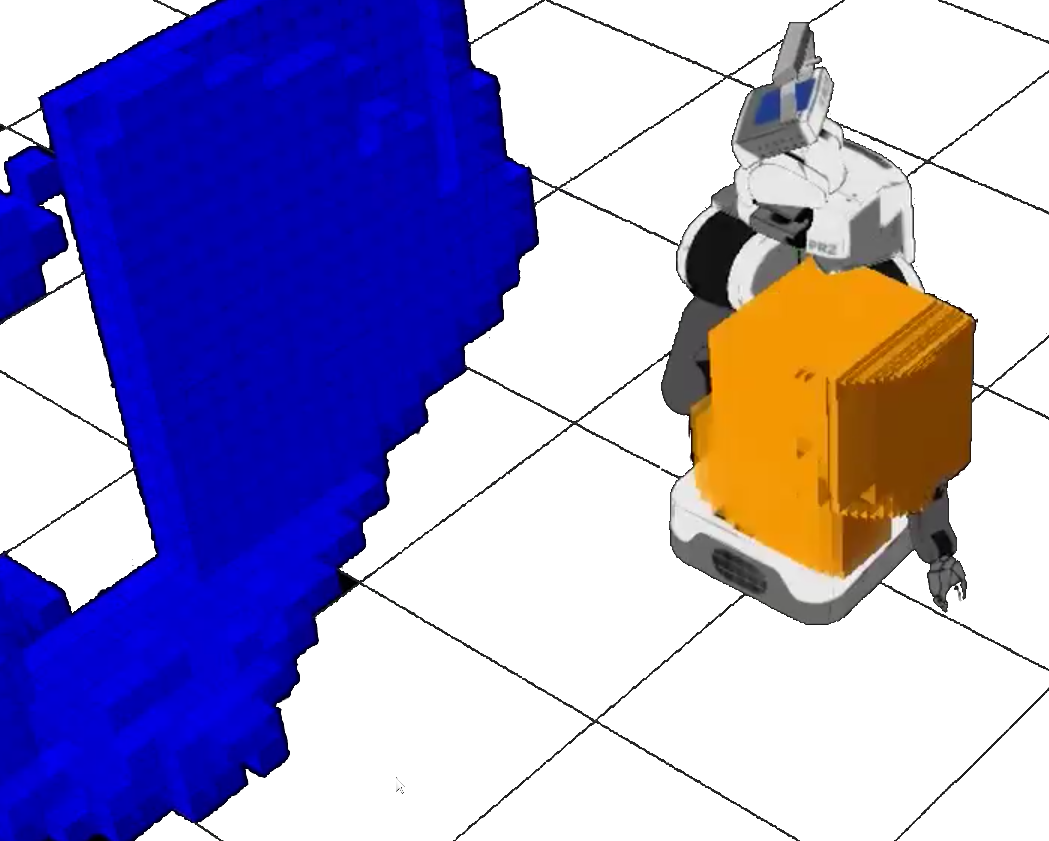
\includegraphics[height=2.1in]{figs/8/unknown2.png}
  \label{fig:8:unknown2}
}
}
\caption[Comparison between the planning algorithms considering and not considering environment uncertainty]{\label{fig:8:unknowncollision} The environment representation can contain unknown
  or uncertain regions in the environment. In the case shown by (a),
  the sensor on the robot's head cannot cover the region near its left
  arm. Therefore, a path for the left arm will always appear
  valid if we ignore unknown regions of the environment and make an optimistic
  assumption, even though obstacles could possibly exist in that
  region. Our solution is shown in (b), where we compute a set of
  boxes (shown in brown) that cover the intersections of robot links
  and unknown parts of the environment. Using these boxes, a notion of
  cost can be easily defined by the user, e.g., using the sum of the occupancy probability of all the boxes. }
\end{figure}





\section{Results}
\label{sec:8:result}

In this section, we present the performance of our new collision checking
and distance computation algorithms when handling the sensor data.

In the first experiment, we use a synthetic \mbox{environment}. First, we
generate $300$ randomly located objects ($100$ spheres, $100$ boxes
and $100$ cylinders). We then construct a dynamic AABB tree broad-phase structure to manage these objects. Next, we randomly generate
an octree structure with $7,784$ cells to simulate the sensor
data. Our task is to perform collision or distance queries between the
dynamic AABB tree and the sensor data. The reported performance for a
single query is the average of the cost for $1,000$ queries. For all experiments on collision query, we compare the overall timing when performing $10$ and $100$ queries. For all experiments on distance query, we only compare the overall timing when performing a single query, because distance query is much more expensive than collision query and thus the time slot for one sensor frame is usually only enough for a single query.

First we compare the performance between our amortized approach and the
traditional non-amortized method and the results are shown in
Table~\ref{table:8:amortized}. We can see that the amortized approach
saves more than $50\%$ of the broad-phase structure construction time,
while the actual collision query is only slightly slower. According to
this result, the amortized approach is faster than traditional methods
when the number of actual queries is $10$ and $100$. As a matter of fact,
the amortized approach is faster than traditional methods
if the number of actual queries is smaller than $38,300$, which is much
larger than the number of collision queries that can be performed during
one sensor data frame.


Next, we compare the performance between the baseline pipeline in~\cite{Rusu:RPG:2009} and our new
pipeline. The results for the collision query are shown in
Table~\ref{table:8:collision}. In
Table~\ref{table:8:collision}(a), all the objects are represented as
primitive shapes; and the octree is also converted into primitive
boxes for the baseline pipeline. In
Table~\ref{table:8:collision}(b), the objects and boxes generated from
octree are in the form of meshes. In the first case, the actual
collision cost in the new pipeline is about two times the cost in the
baseline pipeline, but the saved overhead cost is much larger than the actual query cost of a single
query. As a result, the new pipeline performs better than the baseline
pipeline if the actual number of queries is smaller than $300$. In the
second case, even the cost of a single query in the new pipeline is
smaller than the baseline pipeline. The results for the distance query are
shown in Table~\ref{table:8:distance}. As in the collision case, the
overhead cost is saved in distance query, and the overall performance is improved in the new
pipeline. However, as the distance query is much more expensive than
the collision query, the performance improvement caused by saving the
overhead of data preparation is not as large as in the collision case. Moreover, note that we assume that all the steps in both pipelines can share the data
efficiently, and therefore we can ignore the data transmission overhead
between different \mbox{steps}. For distributed robot systems, such
transmission overhead can be large and therefore we underestimate the
performance improvement caused by the new pipeline, because the new
pipeline has fewer steps than the baseline pipeline.

In the second experiment, we perform collision or distance queries
between a PR2 robot and the sensor data. The PR2 robot has $88$ links,
some in the form of primitive geometric shapes (e.g., cylinders and spheres) and others represented as meshes. The sensor data is an octree with $24,803$ cells. For collision queries, the PR2's average penetration depth into the obstacles is 2.8 $cm$. For distance queries, the PR2's average distance to the obstacles is 3.4 $cm$. Note that collision or distance queries are slow in case of small penetration depth or small distance to the obstacles, since the AABB cannot perform culling effectively in such cases. As a result, the scene is challenging for both collision and distance queries. The results are shown in Table~\ref{table:8:pr2}; we observe similar performance improvements on real-world sensor data with the PR2 robot, as in the synthetic case.

From these results, we can see the difference between the baseline pipeline using the amortized approach and the new pipeline. The amortized approach
only reduces the overhead instead of completely avoiding it, but the
performance reduction on a single actual query is small. The new pipeline completely avoids the overhead, but the time
cost for one actual query may be notably larger than the traditional
pipeline. As a result, the amortized approach is more suitable for
cases where the number of actual queries per sensor frame is large,
e.g., when the environment does not change frequently and the sensor frame rate is
small; or when there are only a few obstacles in the environment. The
method using the new pipeline is more suitable for dynamic
environments with high sensor data frame rates, or for environments with
many obstacles. Moreover, we have observed that the collision query benefits more from our new pipeline than the distance query, since the distance query is usually more expensive and the initialization overhead is less significant. Finally, the speedup caused by the new pipeline is more considerable for scenarios with many obstacles, since the initialization overhead increases with the number of obstacles.

Figure~\ref{fig:8:unknowncollision} shows how a motion planner can use the results provided by our algorithms to improve its performance in environment with unknown/uncertain regions. Given a task, the planner first computes a trajectory that does not collide with the region known to be occupied by obstacles. Then using our methods, we can compute the part of unknown regions that intersect with the robot, which is marked using brown color in Figure~\ref{fig:8:unknowncollision}(b). The motion planner needs more information about these regions in order to determine whether the trajectory is indeed collision-free, which can be performed via various strategies, e.g., to turn the sensor towards the marked region with the maximum entropy. Given the regions with large collision probability, robots can use active sensing to reduce the uncertainty in these regions and therefore improve the execution safety by avoiding collision with objects in these unknown regions, as shown in Figure~\ref{fig:8:actualPR2}.

\begin{figure*}[t]
  \centering
  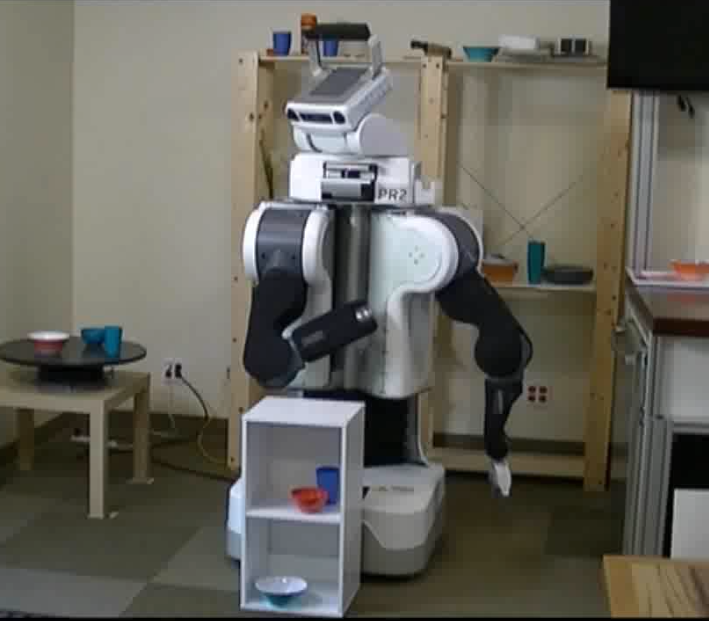
\includegraphics[height=1.8in]{figs/8/fail1.png}
  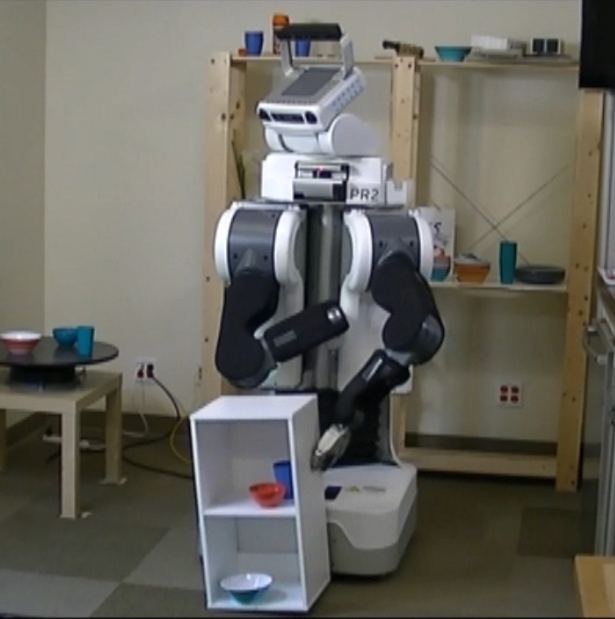
\includegraphics[height=1.8in]{figs/8/fail2.png}
  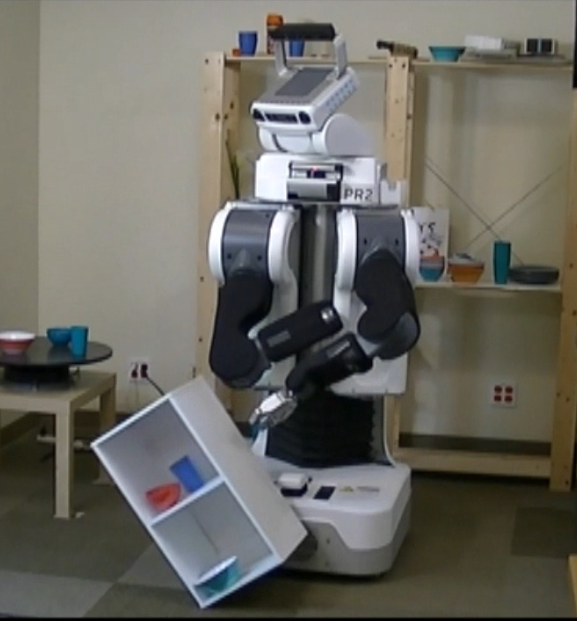
\includegraphics[height=1.8in]{figs/8/fail3.png}
  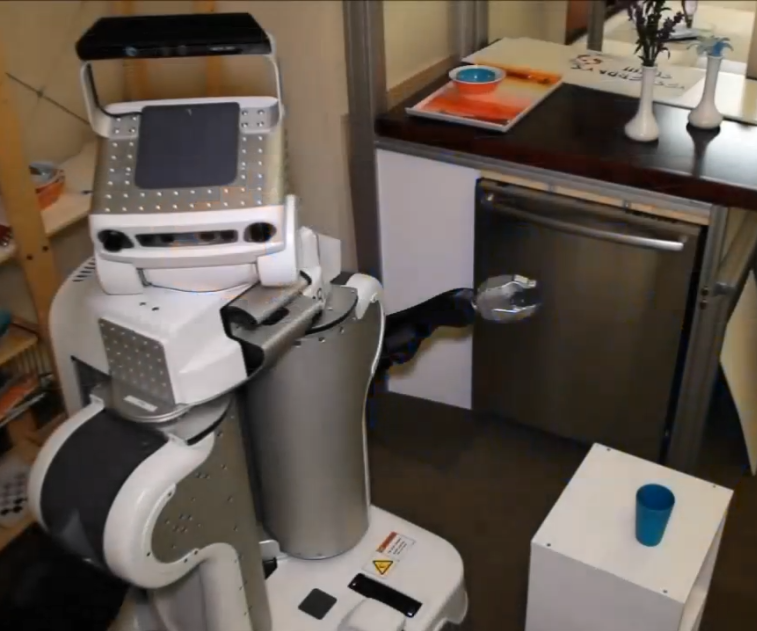
\includegraphics[height=1.2in]{figs/8/succ1.png}
  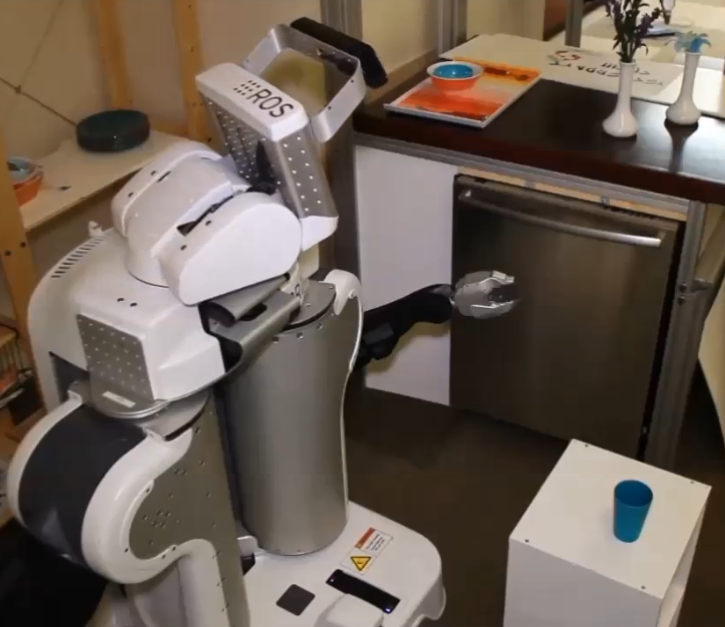
\includegraphics[height=1.2in]{figs/8/succ2.png}
  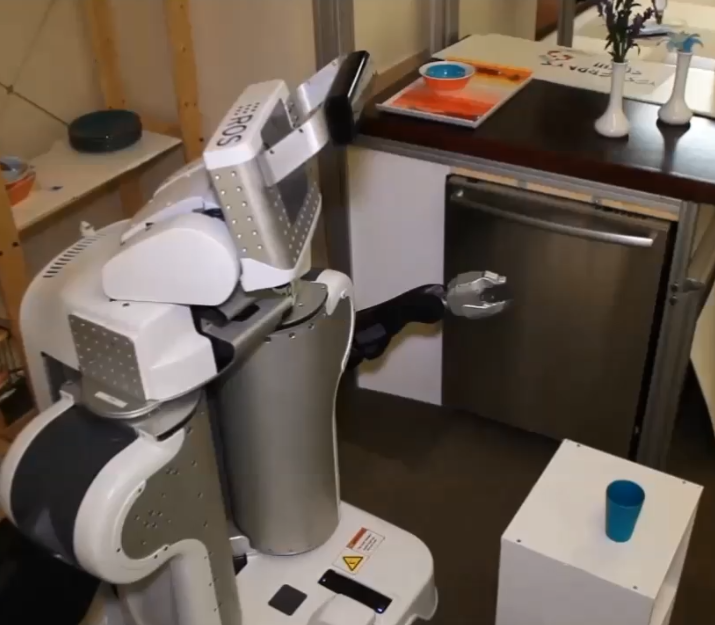
\includegraphics[height=1.2in]{figs/8/succ3.png}
  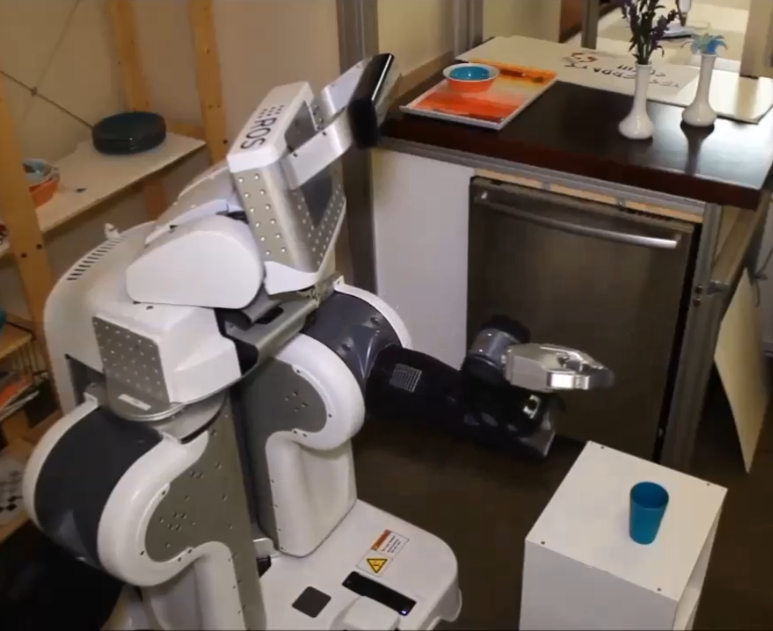
\includegraphics[height=1.2in]{figs/8/succ4.png}
  \caption[Comparison experiments on PR2 robot without and with active sensing]{\label{fig:8:actualPR2} Comparison experiments on PR2 robot without active sensing (first row) and with active sensing (second row). When using active sensing, the robot can safely avoid the cupboard not covered by the initial sensor data.}
\end{figure*}


\begin{table}[htbp]
\centering
\begin{tabular}{c|c c | c c}
 & $T_1$ & $T_q$ & $T_1 + 10 \cdot T_q$ & $T_1 + 10^2 \cdot T_q$ \\\hline
non-amortized & 2.07 & $4.49\cdot 10^{-3}$ & 2.11 & 2.52 \\
amortized & 0.92 & $4.52 \cdot 10^{-3}$ & 0.96 & 1.37 \\
\end{tabular}
\caption[Performance comparison between pipelines with and without amortized broad-phase structure construction]{Performance comparison between baseline pipeline with and without amortized broad-phase structure construction (in ms). The high-quality broad-phase structure computed by non-amortized algorithm improves the total computation only when there are more than $N_{min} = 38333$ collision queries for one frame of sensor data, and the total time required for $N_{min}$ queries is 174 ms, which is much longer than sensor data's update period ($30$ ms for data arriving at 30 Hz).
\label{table:8:amortized}
}
\end{table}

\begin{table}[ht]
\centering
\setlength{\tabcolsep}{4pt}
\subfloat[Objects and boxes are in the form of geometric primitives]{
\begin{tabular}{c|c c c| c c }
 & $T_{1,1}$ & $T_{1,2}$ & $T_q$ & $T_1 + 10 \cdot T_q$ & $T_1 + 10^2 \cdot T_q$ \\\hline
baseline pipeline & 2.283 & 5.389 & 0.022 & 7.89 & 9.872\\
our pipeline & 0 & 0 & 0.048 & 0.48 & 4.8 \\
\end{tabular}}
\\
\subfloat[Objects and boxes are in the form of meshes]{
\begin{tabular}{c|c c c| c c}
 & $T_{1,1}$ & $T_{1,2}$ & $T_q$ & $T_1 + 10 \cdot T_q$ & $T_1 + 10^2 \cdot T_q$ \\\hline
baseline pipeline & 2.697 & 5.465 & 0.317 & 11.3 & 39.9 \\
our pipeline & 0 & 0 & 0.075 & 0.75 & 7.5 \\
\end{tabular}}
\caption[Collision query performance comparison between the baseline pipeline in~\cite{Rusu:RPG:2009} and our new pipeline]{Collision query performance comparison between the baseline pipeline in~\cite{Rusu:RPG:2009} and our new pipeline (in ms). In both pipelines, the $300$ objects in the environment are in the form of primitive geometric shapes or meshes. For the baseline pipeline, the boxes generated from the octree are also represented as primitive boxes or meshes, respectively. When objects are in the form of primitive geometric shapes, the broad-phase structure computed by the baseline algorithm improves the total computation only when there are more than $N_{min} = 2959$ collision queries for one frame of sensor data, and the total time required for $N_{min}$ queries is 72.77 ms, which is much longer than sensor data's update period ($30$ ms for data arriving at 30 Hz). When objects are in the form of meshes, the average query time given by our new pipeline may even be faster the the average query time provided by the baseline pipeline.
\label{table:8:collision}}
\end{table}


\begin{table}[ht]
\centering
\subfloat[Objects and boxes are in the form of geometric primitives]{
\begin{tabular}{c|c c c | c}
 & $T_{1,1}$ & $T_{1,2}$ & $T_q$ & $T_1 + T_q$ \\\hline
baseline pipeline & 2.665 & 5.381 & 23.98 & 32.03 \\
our pipeline & 0 & 0 & 17.40 & 17.40\\
\end{tabular}}
\\
\subfloat[Objects and boxes are in the form of meshes]{
\begin{tabular}{c|c c c | c}
 & $T_{1,1}$ & $T_{1,2}$ & $T_q$ & $T_1 + T_q$ \\\hline
baseline pipeline & 2.871 & 5.413 & 68.03 & 76.31\\
our pipeline & 0 & 0 & 61.86 & 61.86 \\
\end{tabular}}
\caption[Distance query performance comparison between the baseline pipeline in~\cite{Rusu:RPG:2009} and our new pipeline]{Distance query performance comparison between the baseline pipeline in~\cite{Rusu:RPG:2009} and our new pipeline (in ms). In both pipelines, the $300$ objects in the environment are in the form of primitive geometric shapes or meshes. For the baseline pipeline, the boxes generated from the octree are also represented as primitive boxes or meshes, respectively. In this experiment, our new pipeline not only avoids the initialization overhead and also behaves better than the baseline pipeline on average distance query time. This is due to the fact that the octree structure may perform distance culling more efficiently than the hierarchy tree structure.
\label{table:8:distance}}
\end{table}


\begin{table}[ht]
\centering
\subfloat[PR2 collision]{
\begin{tabular}{c|c c | c c}
 & $T_1$ & $T_q$ & $T_1 + 10\cdot T_q$ & $T_1 + 10^2 \cdot T_q$ \\\hline
baseline pipeline & 0.131 & 0.00127 & 0.1437 & 0.258 \\
our pipeline & 0 & 0.00131 & 0.0131 & 0.131 \\
\end{tabular}}
\\
\subfloat[PR2 distance]{
\begin{tabular}{c|c c | c}
 & $T_1$ & $T_q$ & $T_1 + T_q$\\\hline
baseline pipeline & 0.163 & 0.039 & 0.202 \\
our pipeline & 0 & 0.048 & 0.048\\
\end{tabular}}
\caption[Collision and distance query performance comparison between the baseline pipeline in~\cite{Rusu:RPG:2009} and our new pipeline on the PR2 robot]{Collision and distance query performance comparison between the baseline pipeline in~\cite{Rusu:RPG:2009} and our new pipeline on the PR2 robot (in ms). For collision query, the broad-phase structure computed by the baseline algorithm improves the total computation only when there are more than $N_{min} = 3275$ collision queries for one frame of sensor data, and the total time required for $N_{min}$ queries is 4.29 ms. For distance query, the broad-phase structure computed by the baseline algorithm improves the total computation only when there are more than $N_{min} = 18$ collision queries for one frame of sensor data, and the total time required for $N_{min}$ queries is 0.87 ms.
\label{table:8:pr2}}
\end{table}




\section{Conclusions}

We have presented two approaches for efficiently performing collision and distance
queries on sensor data. The first method amortizes the sensor data pre-processing
overhead over all the queries, and is suitable for static or simple
environments. The second method shortens the traditional pipeline by
directly performing queries between the robot links and an octree that
represents sensor data. This approach completely avoids the data
pre-processing overhead, and is suitable for dynamic or complex
environments. We demonstrated the performance of the two methods on
synthetic benchmarks and on environments constructed using the RGB-D
sensor mounted on the PR2 robot. Our new approach also supports
collision queries for sensor data with uncertain or unknown regions.
In summary, the techniques we propose in this chapter will make
collision checking and distance queries with real sensor data more efficient;
will improve the reactive behavior of robots operating in unstructured
environments; and will allow them to deal better with uncertain information
about the environment.

For future work, we are interested in further improving the collision
checking and distance query implementations. We are also interested in
applications of this chapter to motion planning and active sensing, e.g., we would like
to design strategies for gaining more information about uncertain or
unknown parts of the environment.




